\documentclass[]{article}
\usepackage{enumerate, amsmath, amssymb, amsthm, wasysym}
\usepackage[margin=1in]{geometry}
\usepackage[T1]{fontenc}
\usepackage{graphicx}
\DeclareGraphicsExtensions{.png}
\begin{document}

\title{Astronomy C3101 \\ Modern Stellar Astrophysics \\ Homework 4}
\author{Rasmi Elasmar}
\date{Tuesday, December 9, 2014}
\maketitle

\begin{enumerate}[\bfseries Problem 1 -]
\item{
	\textit{Estimating the maximum stellar luminosity}
	\begin{enumerate}
	\item{
		We set the inward gravitational force per unit mass equal to the outward radiative force per unit mass:
		\begin{gather*}
			\frac{GM}{R^2} = \frac{\kappa L}{4 \pi R^2 c}
			\\
			\Rightarrow \frac{M}{L} = \frac{\kappa }{4 \pi c G}
		\end{gather*}
		\\
		Higher mass would favor the inward gravitational force, so we put an upper bound on the left side to indicate that outward radiation pressure dominates and mass may be ejected from the star if this condition is met.
		\begin{gather*}
			\frac{M}{L} < \frac{\kappa }{4 \pi c G}
		\end{gather*}
	}
	\\
	\item{
		With $\kappa = 0.3\, cm^2 \, g^{-1}$, the maximum luminosity  is:
		\begin{gather*}
			L_{max} = \frac{4 \pi c GM}{\kappa}
		\end{gather*}
		Using Wolfram Alpha for some quick calculations,
		\\
		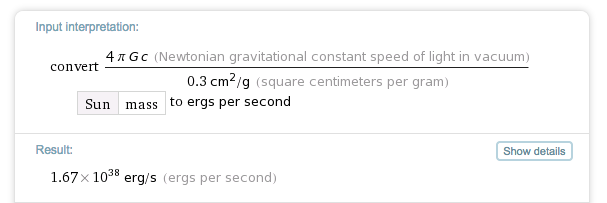
\includegraphics[width=400px]{eddingtonluminosity}
		\\
		Leaving us with 
		\begin{gather*}
			L_{max} = 1.67 \times 10^{38} \frac{M}{M_{\astrosun}} erg/sec
		\end{gather*}
		This is the Eddington Luminosity!
	}
	\item{
		Considering $L_{max}$ from above,
		\begin{gather*}
			\frac{L}{L_{\astrosun}} = \bigg(\frac{M}{M_{\astrosun}}\bigg)^4
			\\
			\Rightarrow \frac{M}{M_{\astrosun}} = \bigg(\frac{L}{L_{\astrosun}}\bigg)^{1/4}
		\end{gather*}
		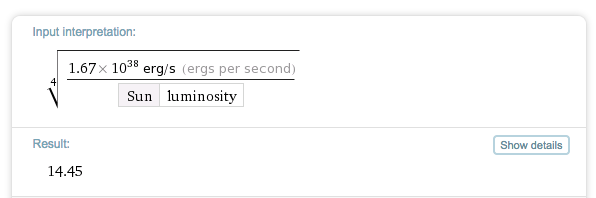
\includegraphics[width=400px]{eddington2}
		\\
		We would need a star of mass $14.45 M_{\astrosun}$ to reach this max luminosity.
		\\
		Looking at the equation in part (b) and fixing $L_{max}$, we would need to increase $\kappa$ to account for an increase in $M$.
	}
	\end{enumerate}
}
\item{
	\textit{Core mass-luminosity relation for RGB stars}
	\begin{gather*}
		L \approx 2.3 \times 10^5 L_{\astrosun} \bigg(\frac{M_c}{M_{\astrosun}}\bigg)^6
	\end{gather*}
	\begin{enumerate}
	\item{
	Core growth $dM_c/dt$ is purely a function of change in mass, and multiplied by energy released per gram (estimated using $e = mc^2$), this gives energy released per unit time (luminosity).
	\\
	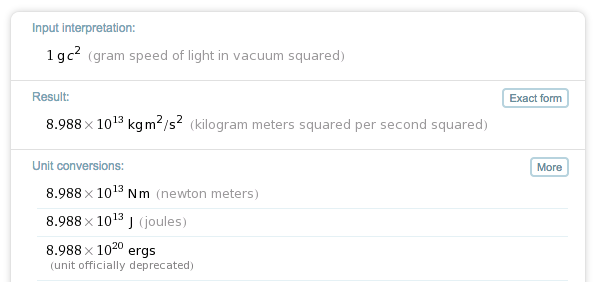
\includegraphics[width=400px]{energy}
	\begin{gather*}
		\frac{dM_c}{dt}(8.988\times 10^{20} ergs) =  L
		\\
		\Rightarrow \frac{dM_c}{dt} =  \frac{2.3 \times 10^5 L_{\astrosun}}{8.988\times 10^{20} ergs}\bigg(\frac{M_c}{M_{\astrosun}}\bigg)^6
	\end{gather*}
	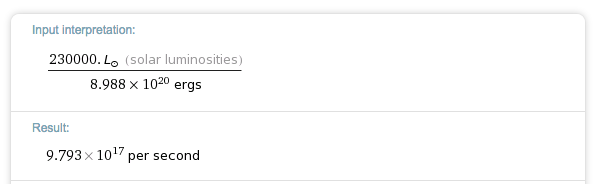
\includegraphics[width=400px]{dmdt}
	Which leaves us with
	\begin{gather*}
		\frac{dM_c}{dt}  = 9.793 \times 10^{17} \big(\frac{M_c}{M_{\astrosun}}\big)^6 g/s
	\end{gather*}
	}
	\item{
	Rearranging to isolate variables then integrating,
	\begin{gather*}
		\frac{dM_c}{M_c^6}  = 9.793 \times 10^{17} \big(\frac{1}{M_{\astrosun}}\big)^6 g/s \cdot dt
		\\
		M_c (t) = -5 M_c^5 \cdot 9.793 \times 10^{17} \big(\frac{1}{M_{\astrosun}}\big)^6 g/s \cdot t
	\end{gather*}
	}
	\item{
	Setting $M_c(t)$ equal to the initial mass of $0.15 M_{\astrosun}$,
	\begin{gather*}
		0.15M_{\astrosun} = -5 (0.15M_{\astrosun})^5 \cdot 9.793 \times 10^{17} \big(\frac{1}{M_{\astrosun}}\big)^6 g/s \cdot t
	\end{gather*}
	Yields $8.021 \times 10^{17} s$.
	\\\\
	Setting $M_c(t)$ equal to the final mass of $0.45 M_{\astrosun}$,
	\begin{gather*}
		0.45M_{\astrosun} = -5 (0.15M_{\astrosun})^5 \cdot 9.793 \times 10^{17} \big(\frac{1}{M_{\astrosun}}\big)^6 g/s \cdot t
	\end{gather*}
	Which yields $t = 2.406 \times 10^{18} s$.
	\\
	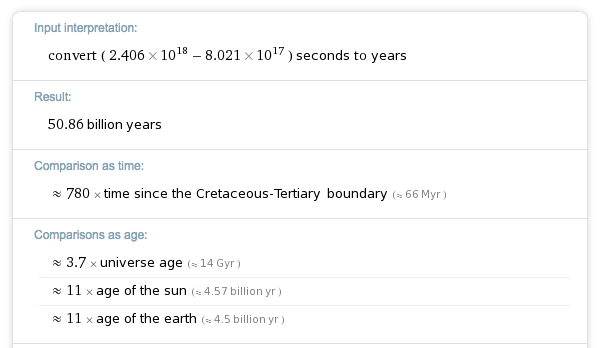
\includegraphics[width=400px]{time1}
	\\\\
	Repeating the process for a $2 M_{\astrosun}$ star yields an entry time of $5.013 \times 10^{16} s$ and exit time of  $7.52 \times 10^{16} s$.
	\\
	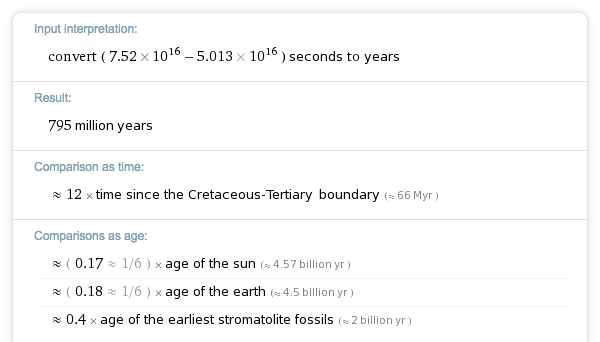
\includegraphics[width=400px]{time2}
	}
	\item{
	When the core reaches $0.45 M_{\astrosun}$, the star shoots up the HR diagram in a flash and ignites Helium burning.
	}
	\item{
	Stars more massive than $2 M_{\astrosun}$ reach the horizontal branch of the HR diagram with Helium burning. Luminosity changes relatively little compared to the increase in temperature.
	}
	\end{enumerate}
}
\item{
	\textit{Mass loss in AGB stars}
	\begin{gather*}
		\dot{M} = -4 \times 10^{-13} \eta \frac{L/L_{\astrosun}}{(g/g_{\astrosun})(R/R_{\astrosun})}M_{\astrosun} yr^{-1}
	\end{gather*}
	\begin{enumerate}
	\item{
	Luminosity is on top because an increase in luminosty would mean a greater decrease in mass (energy is being released). Greater surface gravity acts against this, since it helps bind the star together. A higher radius acts to encourage mass loss because it decreases density.
	}
	\end{enumerate}
}
\item{
	\textit{Yet more STATSTAR fun}
	\\\\
	(see attached)
}
\end{enumerate}
\end{document}
